% !TeX spellcheck = en_US
\section{CrowdCompose}
\label{sec:620_System_Architecture}
The set of filtered video views can either be composed by the semi-automatic composition engine CrowdCompose or the trained model of AutoCompose.
CrowdCompose leverages the concept of crowdsourcing to recruit a large group of human workers, who complete predefined and small tasks to compose a video.
These workers work in parallel on the small jobs and receive a monetary compensation for a successful completion. 

The aim of CrowdCompose is two-fold:
\begin{enumerate}
\item To compose a video stream which achieves a perceived quality superior to existing automatic algorithms, and
\item to create composition models, which can later be used by the automatic composition algorithm AutoCompose.
\end{enumerate}

\subsection{Architecture of CrowdCompose}
Figure~\ref{fig:620_Overview_CrowdDirector} depicts the components required in CrowdCompose, which are distributed across several server instances to cope with a high number of concurrent users composing a video stream.
\begin{figure}[!htb]
\centering
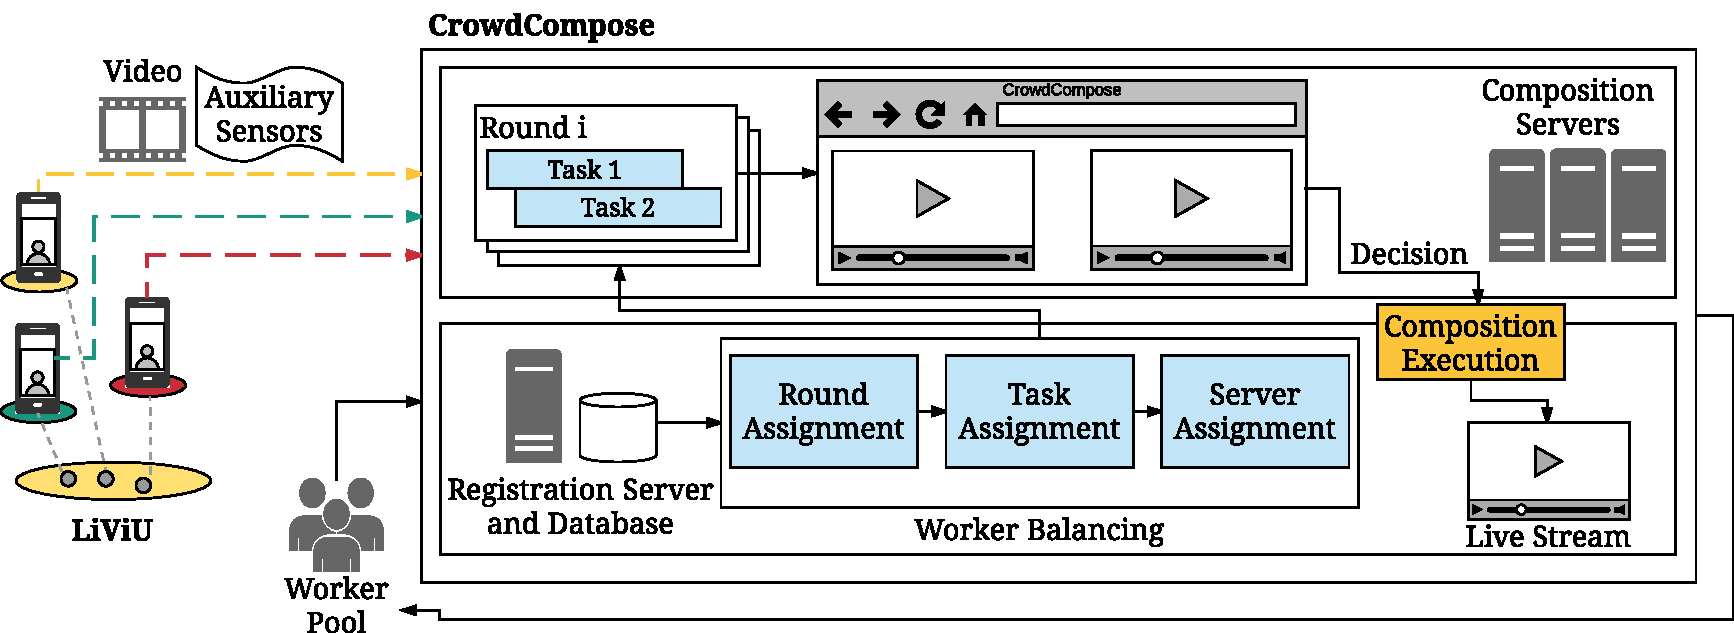
\includegraphics[width=\linewidth]{./gfx/600_Composition/Overview_CrowdDirect}
\caption{Architecture of CrowdCompose for conducting a semi-automatic video composition.}
\label{fig:620_Overview_CrowdDirector}
\end{figure}
\subsubsection{Overview on Different Servers}
CrowdCompose outsources the task of composing live video to a large workforce mediated by an online crowdsourcing platform, such as Microworkers\footnote{www.microworkers.com; Visited on: 09/02/2016}. 
It is assumed that this mediating platform offers a pool of workers which are instantly available to complete tasks.
CrowdCompose assigns tasks to these workers and tries to keep them bound to the system as long as possible.
The service consists of one central \emph{registration server} as well as a scalable number of \emph{composition servers}, which offer the composition \ac{UI}.
The infrastructure implies that all servers are connected by high-speed networks, ensuring both low delay and an exchange of multiple parallel video streams. 
In the current setup of CrowdCompose, this is achieved by deploying all servers in a single data center.
All servers share a dedicated storage on which incoming video views are stored.

\paragraph{Registration Server}
The \emph{registration server} is the initial point of contact for both the workers composing a video stream as well as \ac{LiViU} when it starts streaming a video.
For \ac{LiViU}, the registration server mediates the recording device to the composition server, which receives the video stream.
At any given moment, \ac{LiViU} streams the video to only one server.

For both the workers and the recording devices, the registration server is used to ensure both a load and user balancing across the composition servers.
Furthermore, the registration server is used to execute the video composition by stitching video streams to the composed video.
Thus, the different composition servers submit the workers' decisions to the registration server.
\paragraph{Composition Server and Clients}
The composition servers provide the web client UI. They receive the various  synchronized video streams, segment them, and provide them to the clients in a single UI, which shows up to four video views of the same event in parallel (see Figure~\ref{fig:620_ui_task2}).
The simplistic \ac{UI} design was shown to be beneficial by Lasecki et al.~\cite{Lasecki2011}.
Minimal interactions possibilities are offered to the user to allow workers to focus on a fast task completion.
The respective tasks that are mediated to the workers are discussed in Section~\ref{sec:620_task_desc}.
Decisions made by the workers are transferred to the registration server to execute the video stitching.

As crowdsourcing implies mitigating streams to an anonymous crowd of people that could be located around the world, their Internet connection speeds may vary.
A connection which does not allow one to stream multiple video views without stalling effects would reduce the speed of the composition and may lead to wrong decisions of workers. 
Each session is thus monitored to ensure that solely workers with sufficient network capacity use the system.
This approach is discussed in Section~\ref{sec:620_reliability}.
\subsubsection{Software and Libraries}
A single MySQL\footnote{http://www.mysql.com/; Visited on: 09/02/2016} database handles the storage of decisions and metadata of the streaming clients.
All servers run a Web- (\ac{HTTP}) and Java Application server\footnote{http://tomcat.apache.org/; Visited on: 09/02/2016} that enables running the web-based \ac{UI} and allows inter-server communication.
The web-based \ac{UI} is implemented using standard \ac{HTML} 5 and JavaScript.

Inter-server communication is achieved using \ac{REST} web services, which encapsulate the public functionality of registration and composition servers.
The registration server can access all videos in a shared storage space, which allows quick stitching into the composed video.
The stitching of videos is achieved by using OpenCV 3\footnote{http://opencv.org/; Visited on: 09/02/2016}, the open source framework for computer vision, and the video coding library FFMPEG\footnote{https://ffmpeg.org/; Visited on: 09/02/2016}.

Similar to \ac{LiViU}, it is assumed that \ac{NTP} allows suitable synchronization of different video streams.
The challenge of synchronizing media streams from different sources is intensively discussed in related work~\cite{Guggenberger2015a,Guggenberger2015,Shrestha2007,Shrestha2010b}.
\subsection{Task Design}
\label{sec:620_task_desc}
CrowdCompose pursues the atomization and parallelization of the tasks to 1) select the next, best video view for a composed video, and 2) determine the point in time to switch to this new view. 

A sequential pattern of the two tasks has been chosen in which Task 1 is generally responsible for agreeing on the next video view, whereas Task 2 is in charge of deciding when to switch views. 
\subsubsection{Task 1: Selection of the Best View}
Task 1 is split into two parts discussing the video and the audio track.
Task 1a is assessing the video views and Task 1b the audio tracks. 
Task 1a and 1b rely on assessing based on the \ac{SSCQS} for subjective quality assessment as discussed in Section~\ref{sec:210_subjective_quality}.
As a result, the \ac{MOS} annotates each video view.
\paragraph{Task 1a - Video View Selection}
\emph{Task 1a -  Video View Selection} asks workers to select the most suitable view.
To reduce assessment times, the video stream is segmented into rounds of duration $t_{r}$ (round time). 
The selection is based on up to four synchronously played back video views for $t_{r}$ seconds.
A reference view represents the media stream currently selected for composition.
The reference view is used to normalize ratings across view groups in a round. 
Each view group contains at least two and up to four video views.
The reference view is part of each view group.
Our empirical study determined the maximum number of video views, as it allows users to retrieve the videos in an appropriate size and without the need to scroll\footnote{For the design the mediating platform Microworkers was used which defines the UI size.}.
Thus, at most four parallel views are clustered into view groups identified by an index.
The video views are reduced in size to allow parallel viewing and timely decision making. 
The reference view is highlighted accordingly in the \ac{UI} (see Figure~\ref{fig:620_ui_task2}). 
Assessment of different video views is possible during the playback of a video segment.
The mean of the assessments of the workers is used to select the best view in each round and to annotate it with a quality value (\ac{MOS}).
\paragraph{Task 1b - Audio Track selection}
In \emph{Task 1b - Audio Track Selection}, the appropriate audio stream is selected for the composed video. 
The aim of this approach is to ensure mostly noise-free audio in the composed video. 
Whereas the audio quality assessment algorithms aim at finding compression artifacts or technical degradations in a track, CrowdCompose aims to find noisy and clamorous recordings.

Only a subset of at most four audio streams is selected. 
The location in the scene model is used to determine those views recorded from a central position and that are at a close distance to the \ac{AoI} (scene model: fr, fc or fb).  
Workers are asked to listen to the reference audio track and a single, new audio track - each of at most $\frac{t_{r}}{2}$ seconds.

In comparison to the video part - where diversity is intended - maintaining stability is important for audio.
This has been shown to be beneficial for video composition by Wu et al.~\cite{Wu2015}.
A switch is only invoked if the reference audio track achieves an \ac{MOS} of less than 3.
\subsubsection{Task 2: Timing of a View Transition}
\emph{Task 2: Timing of a view transition} allows workers to give an answer to the question of when to switch from one view to another. 
The \ac{UI} for Task 2 is illustrated in Figure \ref{fig:620_ui_task2}, which includes the reference view on the left and on the right the best-rated video view.
The worker selects the point in time when to switch from the left to the right video view.
\paragraph{User Interface and Selection} 
The timeline at the top shows both the time since task initiation and the decisions of other workers. 
Workers could jump back in time up to $b_c$ seconds and replay the video segment. 
Audio playback stems from the reference video view to determine a comprehensive overview of the best point in time to switch. 
Workers have the possibility to abort a switch from one view to another and thus indicate that the composition should play back the reference video view longer.
\begin{figure}[htb]
\centering
\subfloat[]{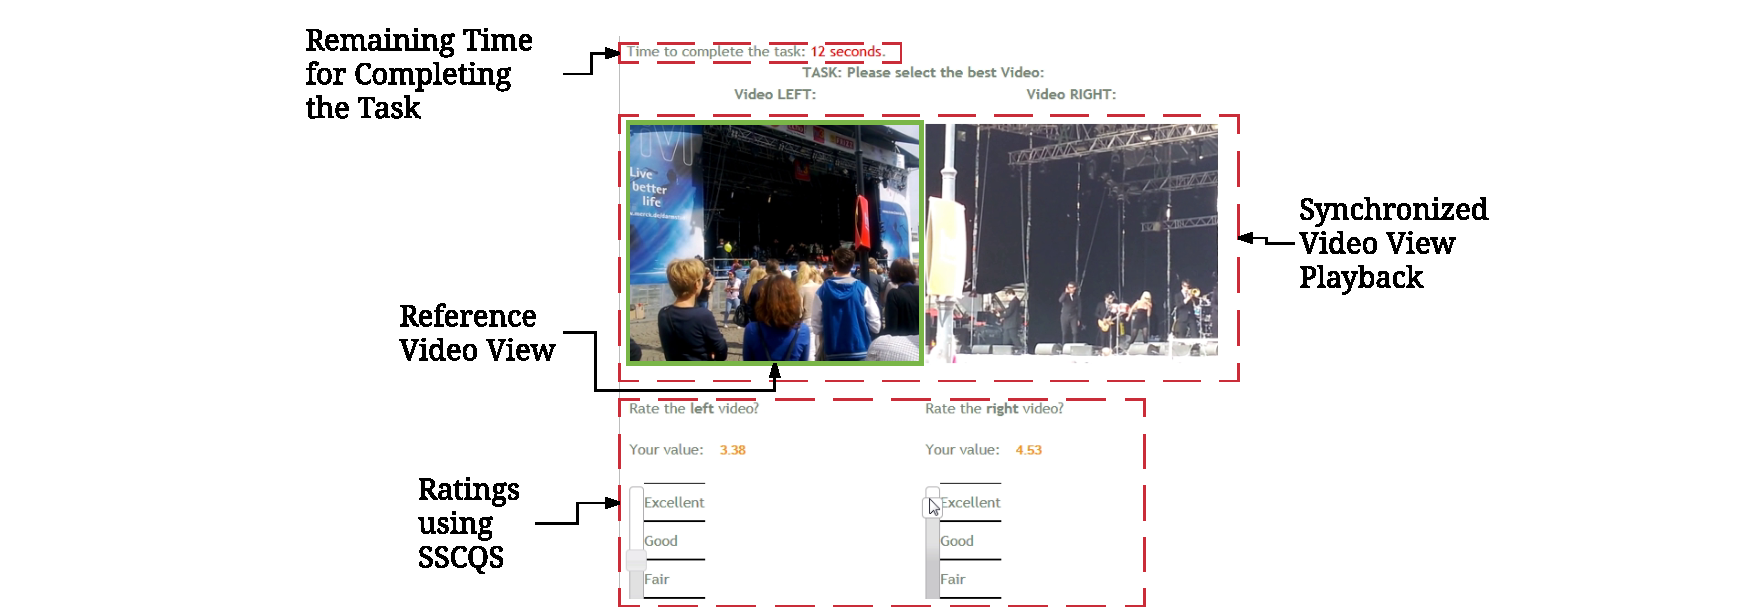
\includegraphics[width=\linewidth]{./gfx/600_Composition/Task1_UI}}\\
\subfloat[]{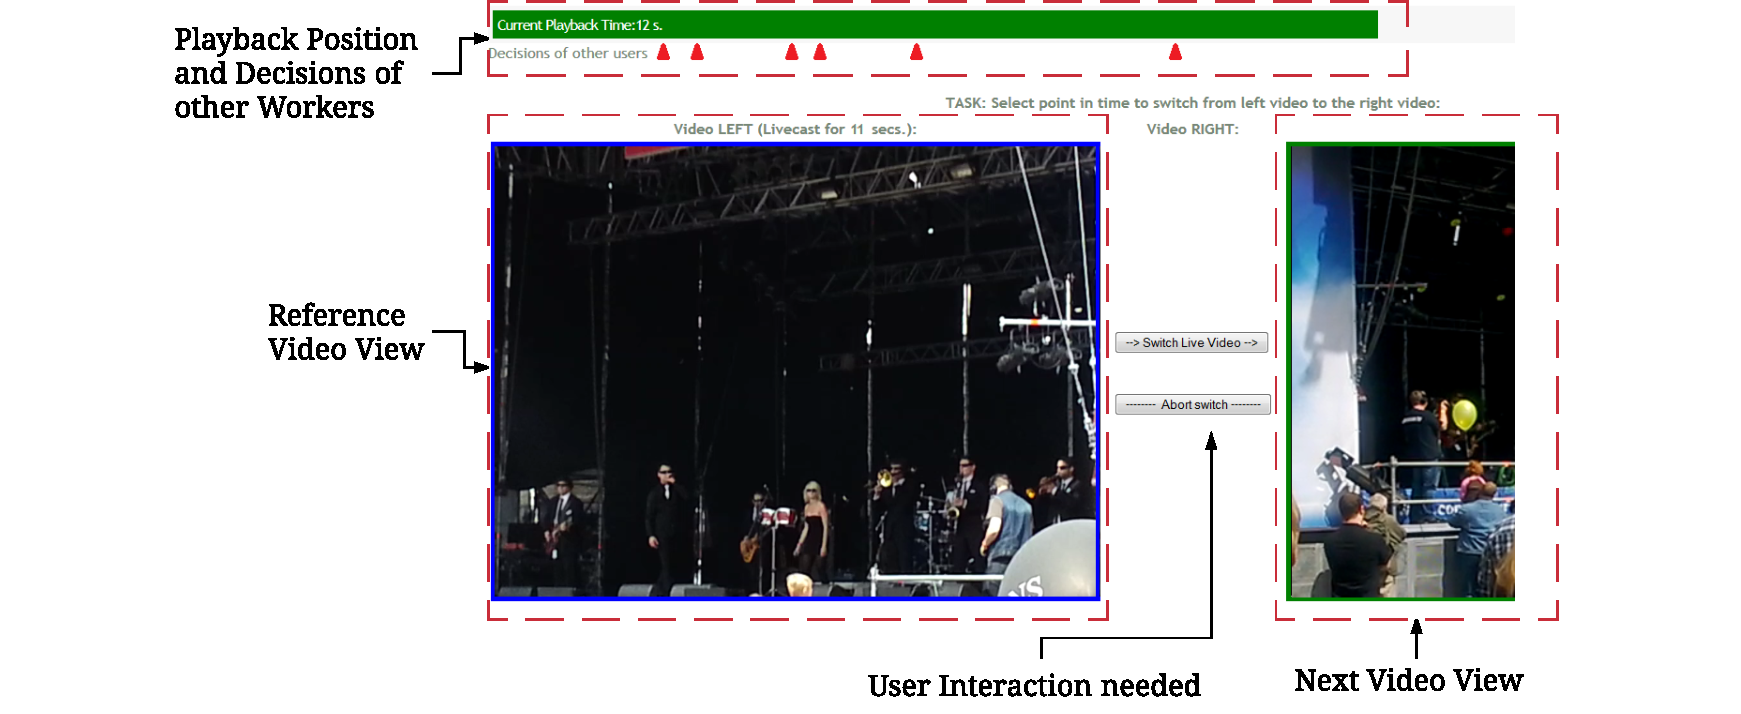
\includegraphics[width=\linewidth]{./gfx/600_Composition/task2_overview_pdf}}
\caption[UI of the different CrowdCompose tasks]{UI of the different CrowdCompose tasks: (a) UI of the CrowdCompose Task 1 - Assessing the quality of video views (b) UI of CrowdCompose Task 2 - Determining the suitable time for a switch in views.}
\label{fig:620_ui_task2}
\end{figure}
If the reference video view is rated best in Task 1a, a switch to the second best-rated view is possible to ensure diverse compositions. 
For Task 2, the total time to find a suitable point for a shot transition is defined by $d_{max} = \overline{d_{G}}+2 \times \sigma d_{G}$, where $d_{G}$ represents a video-genre-dependent threshold (see Section~\ref{sec:690_eval_perceived_quality}).
\paragraph{Refinement of a Decision}
Workers may select very diverse switch points.
This may indicate personal optima for placing a switch, where CrowdCompose needs a collaboratively agreed decision.
To reach a common decision on when a switch shall be placed, a refinement approach is integrated into this task.

CrowdCompose monitors how many workers are currently working on Task 2 and the current time of assessment from a given, synchronized point in time when Task 2 started.
This point in time continuously increases to $d_{max}$.
Every second, it is evaluated if a window of 25\% of the duration can be identified in which a majority of workers agreed on placing a switch.
At least three workers have to place the switch point accordingly.
As soon as this window is identified, the current round for Task 2 is completed, and no further decisions are accepted.

This design is a modified version of the crowdsourcing algorithm "rapid refinement" by Bernstein et al.~\cite{Bernstein2011}. 
In contrast to "rapid refinement", the proposed modification allows workers to see the selections of other workers on a timeline, with the ability to rewind playback and rethink a decision. 
The identified window is then used for a refinement of the task.
Workers repeat the task for the previously determined video segment.
The process is terminated either after two refinements or if a majority of all votes are within a three-second window. 
Video cut points are automatically determined by averaging all human decisions.
No switch is conducted if the majority of workers decided not to switch.
\subsection{Round System and Playback Delay}
Timings and durations are important for understanding CrowdCompose, as the time workers need to make decisions delays the broadcast of a video. 
This delay is known as the broadcast delay and is calculated as $BD = n \times t_{r} + b_c + 5 [s]$ . 

For Task 1a the live stream is divided into segments, called rounds, of $t_{r}$ seconds of video. 
A number of $n$ rounds can be processed in parallel. 
$b_c$ describes the composition buffer in seconds which allows workers to rewind the video in Task 2 for placing a switch. 
Five seconds are reserved for stitching the composed video. 

Increasing values of $t_{r}$ and $n$ delay the creation and playback of the composed video. 
Depending on the timing requirements, which can be specific to the video genre, both parameters $n$ and $t_{r}$ are adjusted (see Section~\ref{sec:690_eval_crowdcompose}). 
Thus, the parameters can be used to define thresholds that workers need to comply with.
If they repeatedly break the given thresholds for executing the tasks, they can be excluded from using the system (see Section~\ref{sec:620_reliability}).
Workers' ratings are discarded if they are not able to complete the task in time. 

\begin{figure}
\centering
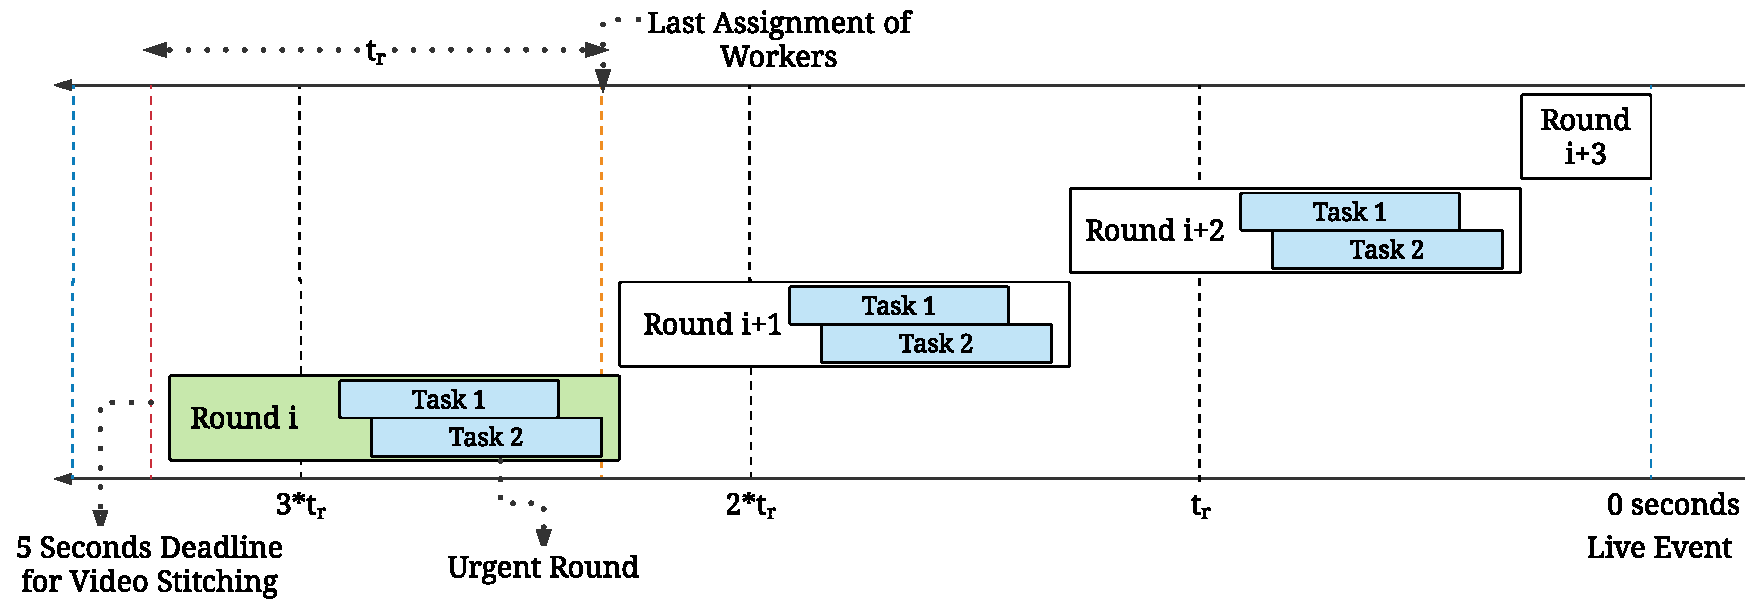
\includegraphics[width=\linewidth]{./gfx/600_Composition/rounds}
\caption[CrowdCompose's round system]{CrowdCompose's round system for parallelizing the video composition.}
\label{fig:620_rounds}
\end{figure}

Figure~\ref{fig:620_rounds} depicts the concepts of in-parallel processing of video streams.
$n$ different rounds are depicted with each containing a fraction of the video stream. 
Five seconds before the broadcast time, the decisions (Task 2) for a round have to be gathered, and the last assignment of workers is consequently possible $t_r + 5$ seconds before the live edge.
$BD$ can thus be adjusted to plan the delay between the reception of a frame on the servers and its distribution to the viewers of a video stream.
\subsection{Worker Balancing}
CrowdCompose integrates automatic balancing of workers across different tasks (see Figure \ref{fig:620_user_assignment}). 
It pipelines workers to conduct the composition in parallel in two ways. 

First, workers are split across different rounds and, second, across different tasks. 
By using this approach, a quick decision can be made when the number of workers is high enough. 
Task assignment prioritizes the evaluation of the video content quality in Task 1a.
After receiving three valid assessments in Task 1a, the assignment of Task 2 is initiated.
 
If more than four parallel video views exist, the views are grouped into view groups, always containing the reference view and three more video streams. 
Each view group is assigned to a distinct CrowdCompose server to ensure an equal server load. 
Balancing checks upon the arrival of a worker if at least three ratings are gathered in the urgent round. 
The urgent round represents the segments for which no final switch decision is made, and which is closest to the live edge.

If this is ensured, the workers are assigned to the rounds in a round-robin manner. 
Groups of three workers are chosen as they allow at each time to retrieve biased assessment. 
To compare the ratings of different view groups, the ratings of the reference view are taken as anchor points. 
\begin{figure}[!htb]
\centering
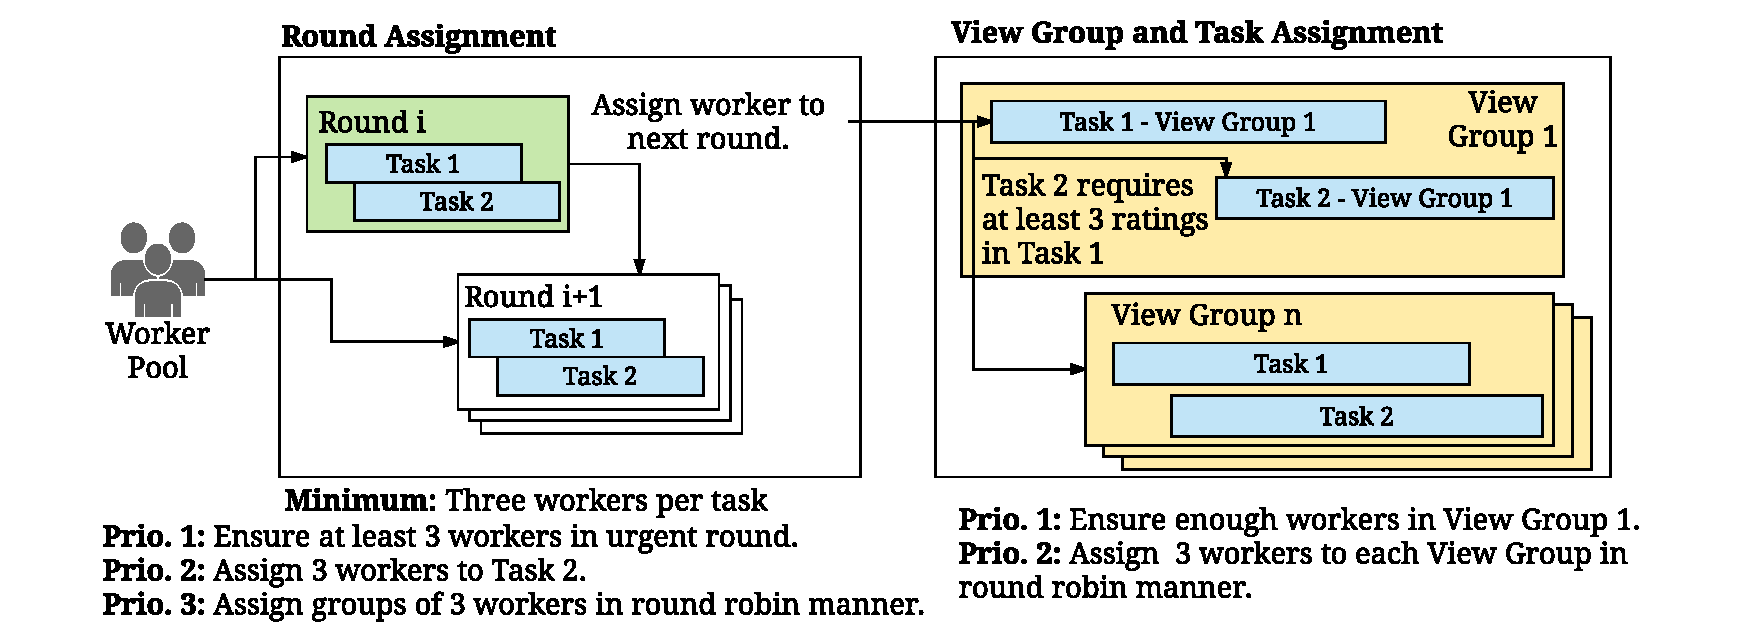
\includegraphics[width=\textwidth]{./gfx/600_Composition/Balancer_simple}
\caption[Worker assignment strategy of CrowdCompose]{Worker assignment strategy of CrowdCompose to different tasks and, if available, view groups.}
\label{fig:620_user_assignment}
\end{figure}
\subsection{Challenges}
Two challenges can occur when using CrowdCompose: a varying number of available users in the worker pool and a varying reliability of the worker's decisions. 
\subsubsection{Varying Workforce}
Mediating crowdsourcing platforms are used to get access to the workforce.
Depending on the time of day the number of workers which start composing a video may change - even within a video composition session.

\paragraph{Queuing in Overcapacity Scenarios}
To compensate for this, the retainer model is used, which keeps workers in the system even though they are not assigned to a task~\cite{Bernstein2011}. 
When a video composition session is initiated, and workers are not immediately assigned to a task, the CrowdCompose website is kept open in a web browser to alert workers when a new task arrives.
As long as the user is queued a minimal compensation is earned per minute - while no task has to be completed.

It is not intended to "over"-assess the views. 
Assessment in Task 1a and 1b is assigned up to $M$ workers per round and task. 
$M$ may range from 3 to 15 or even higher. 
If more than half of the assessors agree on the ranking of the best views, the assignment is stopped.
\paragraph{Skipping Rounds in Undercapacity Scenarios}
If multiple view groups exist and no workforce is available, the completion of all tasks for one view group is favored over a partial processing of all view groups.  
Thus, a decision has to be made which views are selected for evaluation. 

Based on the historic assessments of the previous round, the best views are selected. 
If they are dispersed across different servers, synchronization of the specified views is initiated to allow workers to make assessments on a single server. This is technically achieved as the server shares common storage space.

A switch to an automatic composition can be invoked if not enough workers are available to complete the composition. 
\subsubsection{Reliability and Training of Workers}
\label{sec:620_reliability}
The subjective assessments conducted in CrowdCompose require a reliable assessment from the majority of the workers. 
To ensure that both workers are well trained, and workers who cheat the system are detected, a qualification task is conducted that familiarizes each workers with the different task types. 
Gold standard questions, which ask workers about the content of the video stream, are used in this qualification task; this helps to detect workers who do not pay sufficient attention to the video streams. 
Only workers who achieve 100\% correct answers are assigned to the worker pool of CrowdCompose.

Monitoring of the workers' response times and their assessments is essential in CrowdCompose. 
Regarding response times, too quick responses imply that the worker has not been watching video views, whereas too high ones imply that the worker is not focused. 
Thus, after each round, a threshold is determined by $\overline{t_r} + 2 \times \sigma_{t_r}$ to potentially identify too slow answers. 

If a worker breaks this threshold for two consecutive rounds, they receive a penalty.
Penalties describe an increasing back-off time until the next task assignment for the misbehaving worker. 
After five back-off penalties, the worker is disallowed to contribute to the system. 
The basic principle of CrowdCompose assumes that the majority of workers perform well and that such a mechanism allows for detecting outliers.

As network speeds can highly vary during a streaming session, sessions are continuously monitored. 
Recurring stalling during the composition would slow down the decision process. 
Thus, workers are automatically withdrawn from a round if the stall duration is more than half a round ($\frac{t_r}{2}$ seconds). 
